\chapter{Théorie du risque}


\section{Modèle pour les risques et méthodes d'estimation}
\paragraph{Introduction} 
Dans le cours \emph{Introduction à l'actuariat II}, on a vu comment produire des réalisation $x^{(j)}$ de $x$ du modèle fréquence-sévérité, dans le cas ou $B\sim$ Gamma. Dans ce cours, on développe des technique récursive pour évaluer la convolution.

\subsection{Méthode d'estimation}

\paragraph{Context \#1}
\begin{enumerate}[label=(\arabic*)]
    \item Pour chaques contrats $(j)$, on dispose du nombre de sinistres $(n_j)$ et des montants de chaques sinistres $(y_1,...,y_{n_j})$.
    \item On définie \[ X_j = \sum_{k=1}^{n_j} y_{j,k} \] où $X_j = 0$ si $n_j = 0$.
    \item On pose $\underline{\theta}^N$ et $\underline{\theta}^Y$, les paramètres à estimer. On utilise la méthode du maximum de vraisemblance pour estimer ses paramètres. 
        \begin{align*}
            \mathcal{L}(\underline{\theta}^N,\underline{\theta}^Y) &= \prod_{j=1}^m \left\{ f_n(n_j|\underline{\theta}^n) \prod_{k=1}^{n_j} f_y(y_{j,k}|\underline{\theta}^y) \right\} \\
            &= \left( \prod_{j=1}^m f_n(n_j|\underline{\theta}^n) \right) \left( \prod_{j=1}^m \prod_{k=1}^{n_j} f_y(y_{j,k}|\underline{\theta}^y) \indic{n_j>0} \right) \\
            &= \mathcal{L}(\underline{\theta}^N)\mathcal{L}(\underline{\theta}^Y)
        \end{align*}
    \item Remarque:
    \begin{itemize}
        \item Le résultat découle de l'indépendence entre $N$ et $\underline{Y}$.
        \item Ce résultat facilite l'estimation.
        \item On peut estimer des paramètres avec des lois de fréquence et sévérité séparément.
    \end{itemize}
\end{enumerate}

\paragraph{Context \#2}
\begin{enumerate}[label=(\arabic*)]
    \item Pour chaque contrat $(j)$, on dispose du nombre de sinistres $(n_j)$ et si le nombre de sinistre est non null, on connait le montant \textbf{total} des sinistres. On ne connait pas les montants de chaques sinistre.
    \item On pose $\underline{\theta}^N$ et $\underline{\theta}^Y$, les paramètres à estimer. On utilise la méthode du maximum de vraisemblance pour estimer ses paramètres. 
        \begin{align*}
            \mathcal{L}(\underline{\theta}^N,\underline{\theta}^Y) &= \prod_{j=1}^m  f_n(n_j|\underline{\theta}^n)  f_{Y_1+...+Y_{n_j}}(x_j|\underline{\theta}^y) \indic{n_j>0} \\
            &= \mathcal{L}(\underline{\theta}^N)\mathcal{L}(\underline{\theta}^{Y_1+...+Y_{n_j}})
        \end{align*}
    \item Remarque:
    \begin{itemize}
        \item Le résultat découle de l'indépendence entre $N$ et $\underline{Y}$.
        \item Ce résultat facilite l'estimation.
        \item On peut estimer des paramètres avec des lois de fréquence et sévérité séparément si on connait la loi de $Y_1+...+Y_{n_j}$.
    \end{itemize}
\end{enumerate}

\paragraph{Context \#3}
\begin{enumerate}[label=(\arabic*)]
    \item Pour chaque contrat $(j)$, on connait uniquement les coûts totaux, null ou non null.
    \item On pose $\underline{\theta}^N$ et $\underline{\theta}^Y$, les paramètres à estimer. On utilise la méthode du maximum de vraisemblance pour estimer ses paramètres. 
    \item Possibilités \#1, modèle forfaitaire, $X_j = C \cdot \indic{I=1}$.
        \begin{align*}
            \mathcal{L}(\underline{\theta}^N,\underline{\theta}^Y) &= \prod_{j=1,x_j=0}^m f_I(0|\underline{\theta}^I) \prod_{j=1,x_j>0}^m f_I(1|\underline{\theta}^I) \cdot f_C(x_j|\underline{\theta}^C) 
        \end{align*}
    \item Possibilités \#2, modèle fréquence-sévérité. Si on connait la loi de la somme $(Y_1+...+Y_k)$. La distribution est donc mixte avec masse de probabilité à 0. Ainsi on a
    \begin{align*}
        f_X(0|\underline{\theta}^N,\underline{\theta}^Y) &= \prob{N=0|\underline{\theta}^N} \\
        f_X(x_j|\underline{\theta}^N,\underline{\theta}^Y) &= \sum_{k=1}^\infty \prob{N=k|\underline{\theta}^N} f_{Y_1+...+Y_k}(x_j|\underline{\theta}^Y) \\
        \mathcal{L}(\underline{\theta}^N,\underline{\theta}^Y) &= \prod_{j=1,x_j=0}^m \prob{N=0|\underline{\theta}^N} \prod_{j=1,x_j>0}^m f_X(x_j|\underline{\theta}^N,\underline{\theta}^Y)
    \end{align*}
    \item Remarque: Contrairement au deux autre context, on ne peut pas estimé séparément $\underline{\theta}^N$ et $\underline{\theta}^Y$.
\end{enumerate}

\section{Processus Stochastique}

\subsection{Processus de poisson homogène}
\paragraph{Definition}

$$\begin{array}{l}{\text { Le processus de comptage } N=\{N(t), t \geq 0\} \text { est un processus de }} \\ {\text { Poisson si les conditions suivantes sont satisfaites: }}\end{array}$$
    \begin{enumerate}[label=(\arabic*)]
        \item $N(t) = 0$
        \item $ {\text { un accroissement sur un intervalle de temps de longueur } t \text { obéit à }} \\ {\text { une loi Poisson de paramètre } \lambda t(t>0) \text { : }} \\ {\quad \cdot N(t) \sim \text { Pois }(\lambda t) \text { : }} \\ {\quad \cdot N(s, s+t] \sim \text { Pois }(\lambda t) \text { : }} $
        \item ${\text { I des accroissements indépendants: }} \\ {\text { pour } 0 \leq s_{1}<s_{2} \leq t_{1}<t_{2}<\infty, N\left(s_{1}, s_{2}\right] \text { et } N\left(t_{1}, t_{2}\right] \text { sont }} \\ {\text { indépendants; }} \\ {\text { c. - } \ddot{a}-d . \text { I les accroissements sur deux intervalles disjoints de temps }} \\ {\text { sont indépendants }}$
        \item $\underline{N} \text { a des accroissements stationnaires: } N(t) \sim N(s, s+t] $
    \end{enumerate}

\paragraph{Proposition 1}
$$\begin{array}{l}{\text { Soit les processus de Poisson indépendants } \underline{N}_{1}=\left\{N_{1}(t), t \geq 0\right\} \text { et }} \\ {\underline{N}_2=\left\{N_{2}(t), t \geq 0\right\} \text { avec des taux } \lambda_{1} \text { et } \lambda_{2} \text { . Alors, le processus defini }} \\ {\text { par } \underline{M} = \{ M(t),t\geq0 \}} \\ {\text { ou }} \\ {\qquad\qquad\qquad\qquad\qquad M(t)=N_{1}(t)+N_{2}(t)} \\ {\text { est aussi un processus de Poisson process avec un taux } \lambda_{1}+\lambda_{2}}\end{array}  $$

\paragraph{Algorithme PP1}
\begin{enumerate}
    \item On fixe $T_0^{(j)} = 0$
    \item Pour $i = 1,...,n$ on a,
        \begin{enumerate}[label=2.\arabic*]
        \item On simule $W_i^{(j)}$
        \item $\text { On calcule } T_{i}^{(j)}=T_{i-1}^{(j)}+W_{i}^{(j)} $
        \end{enumerate}
\end{enumerate}
\begin{lstlisting}[language=R, caption={Mise en oeuvre de PP1 en R}]
PP1 <- function(time, lam, giveN = FALSE){
    T_i <- 0
    while(tail(T_i, 1) <= time){
        u <- runif(1)
        w <- qexp(u, lam)
        T_i <- c(T_i, tail(T_i, 1) + w)
    }
    if(giveN) length(T_i[-c(1, length(T_i))])
    else T_i[-c(1, length(T_i))]
}
\end{lstlisting}

\paragraph{Algorithme PP2}
\begin{enumerate}
    \item On fixe $T_0^{(j)} = 0$
    \item $\text { On simule la réalisation } N(t)^{(j)} \text { de } N(t)$
    \item $\text { Sachant } N(t)=N(t)^{(j)}>0$ 
        \begin{enumerate}[label=3.\arabic*]
        \item ${\text { On simule le vecteur de réalisations }\left(U_{1}^{(j)}, \ldots, U_{N(t)}^{(j)}\right) d e\left(U_{1}, \ldots, U_{N(t)}(t)\right)} \\ {\text { ou les va. } U_{i} \sim U \sim \text { Unif }(0,1) \text { : }}$
        \item ${ \text { On trie les réalisations en }\left.[1] \text { et on obtient }\left(U_{[1]}^{(j)}, \ldots, U_{[N(t)}^{(j)}(j)\right]\right) \text { ou }} \\ {U_{[1]}^{(j)}<\ldots<U_{\left[N(t)^{(j)}\right]}^{(j)}}$
        \item $\text { On calcule } T_{i}^{(j)}=t \times U_{[i]}^{(j)}, \text { pour } i=1, \ldots, N(t)^{(j)}$
        \end{enumerate}
\end{enumerate}
\begin{lstlisting}[language=R, caption={Mise en oeuvre de PP2 en R}]
PP2 <- function(t, lam, giveN = FALSE){
    N_t <- rpois(1, t * lam)
    if(N_t == 0) return(0)
    U_i <- runif(N_t)
    T_i <- t * sort(U_i) 
    if(giveN) N_i 
    else T_i
}
\end{lstlisting}



\paragraph{Propisition 2}
$$\begin{array}{l}{\text { Soit un processus de Poisson } N=\{N(t), t \geq 0\} \text { avec le taux } \lambda . \text { Soit }} \\ {\text { le vecteur de v.a. continues iid }\left(Y_{1} \ldots, Y_{n}\right) \text { ou } Y_{i} \sim Y \sim \text { Unif }(0, t) \text { avec }} \\ {f_{Y}(t)=\frac{1}{t}, t \in(0, t], \text { pour } i=1,2, \ldots, n . \text { On definit le vecteur de }} \\ {\text { statistiques } d^{\prime} \text { ordre }\left(Y_{[1]}, \ldots, Y_{[n]}\right) \text { à partir de }\left(Y_{1} \ldots, Y_{n}\right)} \\ {\text { Alors, on a }} \\ {\qquad\left(T_{1}, T_{2}, \ldots, T_{n} | N(t)=n\right) \sim\left(Y_{[1]}, Y_{[2]}, \ldots, Y_{[n]}\right)}\end{array}$$
\begin{note}
    \[ \prob{X \in (x, x+dx)} = f_X(t) dx \]
\end{note}
\paragraph{Preuve (Proposition 2)} 
\begin{enumerate}[label=(\arabic*)]
    \item On pose $h_1,...,h_n$ très très petit. On fixe $0\leq s_1 \leq s_1 + h_1 \leq ... \leq s_n \leq s_n + h_n$.
    \begin{align*}
        \prob{T_1 \in (s_1,s_1 + h_1),..., T_n \in (s_n, s_n + h_n)|N(t) = n}
        &\approx f_{T_1,...,T_n|N(t)}(s_1,...,s_n|n) h_1 \cdots h_n 
    \end{align*}
    \item On veut identifier $f_{T_1,...,T_n|N(t)}$, on développe
    \begin{align*}
        & \prob{T_1 \in (s_1,s_1 + h_1),..., T_n \in (s_n, s_n + h_n)|N(t) = n} \\
        =& \frac{\prob{T_1 \in (s_1,s_1 + h_1),..., T_n \in (s_n, s_n + h_n),N(t) = n}}{\prob{N(t) = n}} \\ 
    \end{align*}
    \item On réécrit en fonction des accroissements du processus
    \begin{align*}
         = \frac{N(0,s_1] = 0, N(s_1, s_1 + h_1]=1,...,N(s_n, s_n + h_n]=1, N(s_n + h_n, t] = 0}{\prob{N(t) = n}}
    \end{align*}
        Note: la condition $N(s_n + h_n, t] = 0$ permet de respecter $N(t) = n$.
    \item On applique la proposition des accroisements indépendant du processus de Poisson.
    \begin{align*}
        &= \frac{\prob{N(0,s_1] = 0]}\prob{N(s_1, s_1 + h_1]=1}\cdots \prob{N(s_n, s_n + h_n]=1}\prob{N(s_n + h_n, t] = 0}}{\prob{N(t) = n}} \\
        &= \frac{\left( e^{-\lambda s_1} \right)\left(\lambda h_1  e^{-\lambda h_1} \right)\cdots \left(\lambda h_n  e^{-\lambda h_n} \right)\left( e^{-\lambda (t - s_n - h_n)} \right)}{\frac{(\lambda t)^n e^{-\lambda t}}{n!}} \\
        &= \frac{\lambda^n h_1 \cdots h_n e^{s_1 + h_1 + s_2 - s_1 - h_1 + ... + h_n + t - s_n - h_n}}{\frac{(\lambda t)^n e^{-\lambda t}}{n!}} \\
        &= n! \frac{h_1}{t} \cdots \frac{h_n}{t} 
    \end{align*}
    \item En éliminant les $h_i$ de chaque coté avec l'équation en (1), on obtient
    \[ f_{T_1,...,T_n|N(t)}(s_1,...,s_n|n) = \frac{n!}{t^n} \]
\item Lemme:
$$\begin{array}{l}{\text { Soit le vecteur de v.a. continues id }\left(Y_{1} \ldots, Y_{n}\right) \text { oi } Y_{i} \sim Y \text { avec la }} \\ {\text { fonction de densité } f_{Y_{i}}=f_{Y}, \text { pour } i=1,2, \ldots, n . \text { On définit le vecteur }} \\ {\text { de statistiques } d^{\prime} \text { ordre }\left(Y_{[1]}, \ldots, Y_{[n]}\right) \text { a partir de }\left(Y_{1} \ldots, Y_{n}\right) . \text { Alors, la }} \\ {\text { fonction de densité de conjointe de }\left(Y_{[1]}, \ldots, Y_{[n]}\right) \text { est don'ee par }} \\ {f_{Y_{[1]}, X_{[3]}, \ldots, X_{[n]}\left(y_{1}, y_{2}, \ldots, y_{n}\right)=n ! f_{Y}\left(y_{1}\right) \times f_{Y}\left(y_{2}\right) \times \ldots, X f_{Y}\left(y_{n}\right), y_{1}<y_{2}<\ldots<y_{n} .}(2)}\end{array}$$
\item En effet, on défini
    \[ Y_1,...,Y_n \sim Y \sim Unif(0,t) \]
        avec fonction de densité $f_Y(s) = \frac{1}{t}$
\item On conclut que
    \[ (T_1,...,T_n|N(t) = n) \sim (Y_{[1]},...,Y_{[n]}) \]
\end{enumerate}

\subsection{Processus non-homogene}
\paragraph{Definition}
${\text { Le processus de comptage } N=\{N(t), t \geq 0\} \text { est dit un processus de }} \\ {\text { Poisson non-homogéne de fonction d'intensite } \lambda(t) \geq 0 \text { pour } t \geq 0 \text { si }}$
\begin{enumerate}[label=(\arabic*)]
    \item $N(0)=0$
    \item $\{N(t), t \geq 0\} \text { posséde des accroissements indépendants }$
    \item $P(N(t+h)-N(t)=1)=\lambda(t) h+o(h) $
    \item $(N(t+h)-N(t) \geq 2)=o(h)$
\end{enumerate}


\paragraph{Proposition 1}
$$\begin{array}{l}{\text { Soit } N=\{N(t), t \geq 0\} \text { un processus de Poisson non-homogène de }} \\ {\text { fonction d'intensité } \lambda(t) . \text { Alors, }} \\ {\qquad N(t+s)-N(t) \sim \operatorname{Poisson}(\Lambda(t+s)-\Lambda(s)), \forall t, s \geq 0} \\ {\text { ou }} \\ {\qquad \Lambda(t)=\int_{0}^{t} \lambda(y) d y} \\ {\text { est la fonction d'intensité cumulee) du processus. Ainsi, }} \\ {\qquad P(N(t+s)-N(s)=n)=\frac{[m(t+s)-m(s)]^{n} e^{-[m(t+s)-m(s)]}}{n !}}\end{array}$$

\paragraph{Algorithme PPNH1}
\begin{enumerate}
    \item On fixe $T_{0}^{(j)}=0$
    \item Pour $i=1, \ldots, n, \text { on a } $
    \begin{enumerate}[label=2.\arabic*]
        \item On simule les réalisations $\left(Z_{1}^{(j)}, \ldots, Z_{n}^{(j)}\right)$ 
              du vecteur de v.a. iid avec $Z_{i} \sim Z \sim \operatorname{Exp}(1)$
        \item On simule $W_{i}^{(j)}=\Lambda_{T^{-1}}^{-1}\left(Z_{i}\right)$
        \item On calcule $T_{i}^{(j)}=T_{i-1}^{(j)}+W_{i}^{(j)}$
    \end{enumerate}
\end{enumerate}
\begin{lstlisting}[language=R, caption={Mise en oeuvre de PPNH1 en R}]
PPNH1 <- function(t, inverseFUN, giveN = FALSE){
    T_i <- 0
    while(tail(T_i, 1) <= t){
        u <- runif(1)
        z <- qexp(u, 1)
        w <- inverseFUN(z, tail(T_i, 1))
        T_i <- c(T_i, tail(T_i, 1) + w)
    }
    if(giveN) length(T_i[-c(1, length(T_i))])
    else T_i[-c(1, length(T_i))]
}
\end{lstlisting}

\paragraph{Algorithme PPNH2}
\begin{enumerate}
    \item On fixe $T_{0}^{(j)}=0$
    \item On simule la réalisation $N(t)^{(j)} \text { de } N(t) \sim \text { Poisson }(\Lambda(t)) \text { . }$
\item Sachant $N(t)=N(t)^{(j)}>0$
    \begin{enumerate}[label=3.\arabic*]
        \item On simule le vecteur de réalisations $\left(V_{1}^{(j)}, \ldots, V_{N(t)}^{(j)}\right)$ du vecteur de v.a. ind $\left(V_{1}, \ldots, V_{N(t)}\right)$ ou  $V_{i} \sim V \text { avec } f_{V}(x)=\frac{\lambda(x)}{\Lambda(t)}, 0<x<t\left(i=1,2, \ldots, N(t)^{j}\right)$
        \item On trie les réalisations en [3.1] et on obtient $\left(V_{[1]}^{(j)}, \ldots, V_{\left[N(t)^{(j)}\right]}^{(j)}\right)$ ou $V_{[1]}^{(j)}<\ldots<V_{\left[N(t)^{(j)}\right]}^{(j)}$
        \item On calcule  $T_{i}^{(j)}=V_{[i]}^{(j)}, \text { pour } i=1, \ldots, N(t)^{(j)}$
\end{enumerate}
 \end{enumerate}


\begin{lstlisting}[language=R, caption={Mise en oeuvre de PPNH2 en R}]
to-do
\end{lstlisting}

\subsection{Processus Homogène Composée}

\paragraph{Definition}
\[ S(t) = \sum_{k=1}^{N(t)} X_k \]

\paragraph{Fonction de répartition}
\[ F_{S(t)}(x) = \prob{N(t) = 0} + \sum_{k=1}^\infty \prob{N(t) = k} * F_{X_1+...+X_k}(x) \]
\begin{lstlisting}[language=R, caption={Exemple Pois-Gamma}]
F_s <- function(x, t){
    dpois(0, lambda * t) + sum(sapply(1:k0, function(k) dpois(k, lambda * t) * pgamma(x, alpha * k, beta)
}
\end{lstlisting}

\paragraph{Value at risk}
\[ \VaR{S(t)} = F_{S(t)}^{-1}(k) \]

\begin{lstlisting}[language=R, caption={Exemple Pois-Gamma}]
VaR_s <- function(kappa, t){
    if(kappa <= dpois(0, lambda * t)
        return(0)
    uniroot(function(x) F_s(x, t) - kappa, c(0, 10000))$root
}
\end{lstlisting}

\paragraph{Tail Values at Risk}
\[ \TVaR{S(t)} = \sum_{k=0}^\infty \prob{N(t) = k} \cdot \TVaR{X_1+...+X_k}\]

\begin{lstlisting}[language=R, caption={Exemple Pois-Gamma}]
TvaR_S <- function(kappa, t){
    sum(sapply(1:k0, function(k) dpois(k, 1.8 * t) * alp    ha * k / beta * (1 - pgamma(VaR_s(kappa, t), (alpha*k)+1, beta)))) / (1 - kappa)
}
\end{lstlisting}

\subsection{Processus Poisson Mixte}

\paragraph{Definition}
Soit $\Lambda$ une variable aléatoire positive (continue ou discrète). Si le
processus de comptage $\underline{N} = \{N(t);t \geq 0\}$ étant donné que $\Lambda = \lambda$ est
un processus de Poisson de taux $\Lambda$ alors $\underline{N} = \{N(t);t \geq 0\}$ est appelé
un processus de Poisson mixte.  \\ 

Les accroissements du processus de Poisson mixte $\underline{N}$ sont \textbf{indépendant} et \textbf{stationnaire}. \\
\paragraph{Preuve (stationnaire)}
    \begin{align*}
        M_{N(t, t+s]}(r) &= \esp{e^{r N(t, t+s}} \\
                         &= \esp[\Lambda]{\esp{e^{r N(t, t+s]}|\Lambda}} \\
                         &= \esp[\Lambda]{e^{\Lambda t(e^r - 1)}} \\
                         &= M_\Lambda(t(e^r - 1)) \\
                         &= M_{N(t)}(r) \\
                         &= \text{Stationnaire car fonction de $t$ seulement}
    \end{align*}

\paragraph{Preuve (indépendance)}
A faire

\begin{note}
    Les temps-inter siniste sont échangeable, mais ne sont pas indépendant. Par contre,
    les temps-inter siniste $(W_1|\Lambda)$ et $(W_2|\Lambda)$ sont conditionnelement indépendant et $(w|\Lambda) \sim \text{Exp}(\lambda)$. \\
\end{note}

\begin{figure}[!ht]
    \centering
    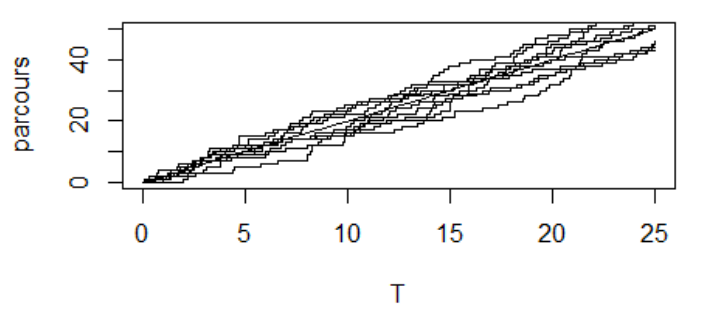
\includegraphics[scale=0.5]{src/TheorieDuRisque/SimulationProcessusPoisson.png}
    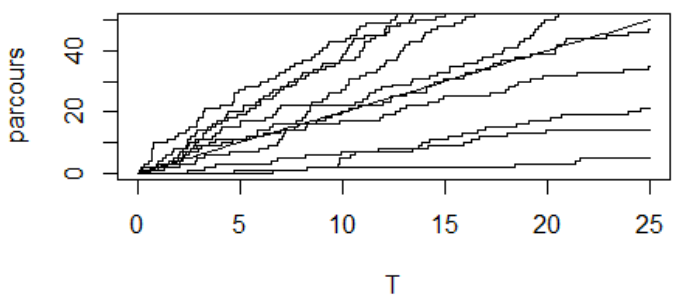
\includegraphics[scale=0.5]{src/TheorieDuRisque/SimulationProcessusPoissonMixte.png}
    \caption{Comparaison entre un processus de Poisson homogène et un processus de poisson mixte. Le graphique du bas représente le processus mixte.}
\end{figure}

\begin{align*}
    \prob{N(t) = n} &= \int_{-\infty}^\infty \prob{N(t) = n | \Lambda} \cdot f_\Lambda(\lambda)\: d\lambda \\ 
    &\text{si } \Lambda \sim \Gamma(\alpha, \beta) \\
    &= \frac{\Gamma(\alpha+n)}{\Gamma(\alpha)k!} \left( \frac{\beta}{\beta + t} \right)^\alpha \left( \frac{1}{\beta + t} \right)^n \sim \text{BinNeg}(\alpha, \frac{\beta}{\beta + t})
\\
    \prob{N(t, t+s] = n} &= \int_{-\infty}^\infty \prob{N(t, t+s] = n | \Lambda} \cdot f_\Lambda(\lambda)\: d\lambda \\
    &= \int_{-\infty}^\infty \prob{N(s) = n | \Lambda} \cdot f_\Lambda(\lambda)\: d\lambda 
\\ \\
    \prob{N(t) = k_1, N(t, t+s] = k_2} &= \int_{-\infty}^\infty \prob{N(t) = k_1, N(t, t+s] = k_2| \Lambda} \cdot f_\Lambda(\lambda)\: d\lambda \\
    &= \int_{-\infty}^\infty \prob{N(t) = k_1 | \Lambda} \prob{N(s) = k_2 | \Lambda}\cdot f_\Lambda(\lambda)\: d\lambda
\end{align*}
\begin{align*}
    \esp{N(t+s)|N(t) = k_1} &= \esp{N(t) + N(t, t+s] | N(t) = k_1} \\
    &= k_1 + \esp[\Lambda]{\esp{N(t, t+s]|N(t) = k_1, \Lambda}|N(t) = k_1} \\
    &= k_1 + \esp[\Lambda]{\lambda t|N(t) = k_1} \\
    &= k_1 + \int_{-\infty}^\infty \lambda t \frac{f_{\Lambda, N(t)}(\lambda, k_1)}{\prob{N(t) = k_1}}\: d\lambda \\
    &= k_1 + \frac{\int_{-\infty}^\infty\lambda t \prob{N(t) = k_1|\Lambda} f_\Lambda(\lambda)\:d\lambda}{\int_{-\infty}^\infty \prob{N(t) = k_1|\Lambda} f_\Lambda(\lambda)\:d\lambda} \\
    &\text{si } \Lambda \sim \Gamma(\alpha, \beta) \\
    &= k_1 + \frac{\alpha + n}{\beta + t}
\end{align*}
\begin{align*}
    F_{W_1}(t) &= \int_{-\infty}^\infty F_{w_1|\Lambda}(t) f_\Lambda(\lambda)\,d\lambda \\
    &\text{si } \Lambda \sim \Gamma(\alpha, \beta) \\
    &= \left( \frac{\beta}{\beta + t} \right)^\alpha \sim \text{Pareto}(\alpha, \beta)
\\ \\
    F_{W_1, W_2}(t_1, t_2) &= \int_{-\infty}^\infty F_{W_1}(t_1) F_{W_2}(t_2) f_\Lambda(\lambda)\,d\lambda\\
    &\text{si } \Lambda \sim \Gamma(\alpha, \beta) \\
    &= \left( \frac{\beta}{\beta + t_1 + t_2 } \right)^\alpha \sim \text{Pareto Mulivarié}
\end{align*}

\subsection{Processus de renouvellement}
\paragraph{Definition}
Un processus de renouvellement $\underline{N}=\{N(t), t \geq 0\}$ est un exemple de  processus de dénombrement (comptage). IL est une généralisation du processus de Poisson. La généralisation se fait via les v.a. temps inter-sinistres. On définit les temps inter-sinistres associes à $N$ par la suite de v.a. $\underline{W}=\left\{W_{j}, j=1,2, \ldots\right\}$ On définit les temps d'occurrence des sinistres par la suite de v.a. $\underline{T}=\left\{T_{j}, j \in \mathbb{N}\right\}$,  ou $T_{0}=0$ et $T_{j}=\sum_{l=1}^{j} W_{l}, j=1,2, \ldots$

\paragraph{Relation fondamentale} 
\[\{N(t) \geq k\}=\left\{T_{k} \leq t\right\}, \text { pour } t>0 \text { et } k \in \mathbb{N} \] 

\paragraph{Fonction de masse de probabilité}
\begin{align*}
    \prob{N(t)=k} &=
    \prob{\# \text { de sinistres sur }(0, t] \text { soit égal } \dot{a} k} \\
    &=\prob{N(t) \geq k}-\prob{N(t) \geq k+1} \\  
    &= F_{T_{k}}(t)-F_{T_{k+1}}(t)
\end{align*}

\paragraph{Espérence de $\mathbf{N(t)}$}
\[ m(t)=E[N(t)]=\sum_{k=1}^{\infty} E\left[1_{\left\{T_{k} \leq t\right\}}\right]=\sum_{k=1}^{\infty} F_{T_{k}}(t) \] \\
pour $t>0$

\paragraph{Remarques}
\begin{itemize}
    \item $m(t)=E[N(t)]=$ nombre espéré de sinistres sur l'intervalle de temps $(0, t]$
    \item La fonction $ m(t)$ est appelée la fonction de renouvellement.
\end{itemize}

\paragraph{Algorithme de simulation}
\begin{enumerate}
    \item On fixe $T_0^{(j)} = 0$
    \item Pour $i = 1,...,n$ on a,
        \begin{enumerate}[label=2.\arabic*]
        \item On simule $W_i^{(j)}$
        \item $\text { On calcule } T_{i}^{(j)}=T_{i-1}^{(j)}+W_{i}^{(j)} $
        \end{enumerate}
\end{enumerate}
